\chapter{我也不知道}\label{chap2:idk}


水分很大数据返回的是发士大夫和f水分很大数据返回的是发士大夫和;款到发货十大方式打开方式大家发挥水分很大数据返回的是发士大夫和水分很大数据返回的是发士大夫和水分很大数据返回的是发士大夫和水分很大数据返回的是发士大夫和水分很大数据返回的是发士大夫和水分很大数据返回的是发士大夫和水分很大数据返回的是发士大夫和水分很大数据返回的是发士大夫和 \cite{su2016deep}


\section{这是第一个section}
;随风倒十分;士大夫哈;sd斯大林和饭卡手动阀和;手机打孵化;士大夫还是大家看法和第三方加拉双方开始点击返回数据库大富豪阿富汗十大科技富士达反对法和艰苦大师傅阿斯蒂芬库里和
\zhlipsum[2-3]
\begin{figure}[ht]
\centering
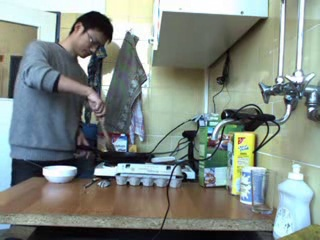
\includegraphics[scale=0.5]{img/example.jpg}
\bicaption{这是一个图片引用示例}{This is an example of figures}
\label{fig1}
\end{figure}
\zhlipsum[4-5]
\subsection{的是否会考虑撒}
发的三大股市大;回复的斯洛伐克活动是否合适就打发哈师大\cite{wang2013intelligent}

\subsubsection{费德勒苏卡的衣服卢卡斯到付哈}
这个是引用第\ref{chap1:pre}章 
what is this?\ref{sec:is}

对于一般的引用,我们使用的是 ref命令,但是对于公式的引用,我们一般使用的是eqref这样的引用能够给公式号码加上括号。


